\documentclass[10pt,letterpaper]{article}
\usepackage{graphicx}
\usepackage[margin=0.8in]{geometry}
\pagestyle{empty}

\begin{document}
\centerline{\Large \bf replicate-1, mutvir}
\vspace{0.1in}

\centerline{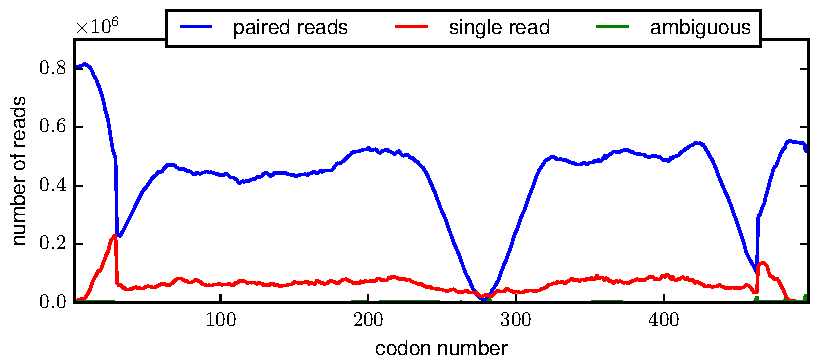
\includegraphics[width=5in]{replicate-1-mutvir_codondepth.pdf}}
\vspace{0.1in}

\centerline{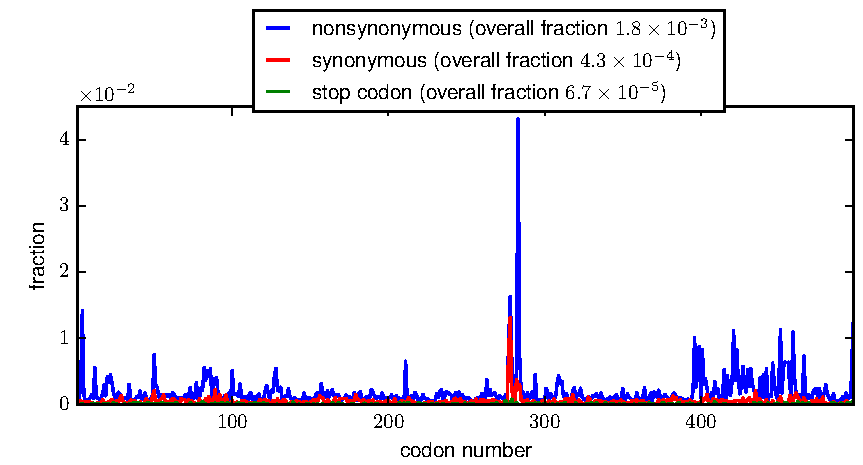
\includegraphics[width=5in]{replicate-1-mutvir_syn-ns-dist.pdf}}
\vspace{0.1in}

\centerline{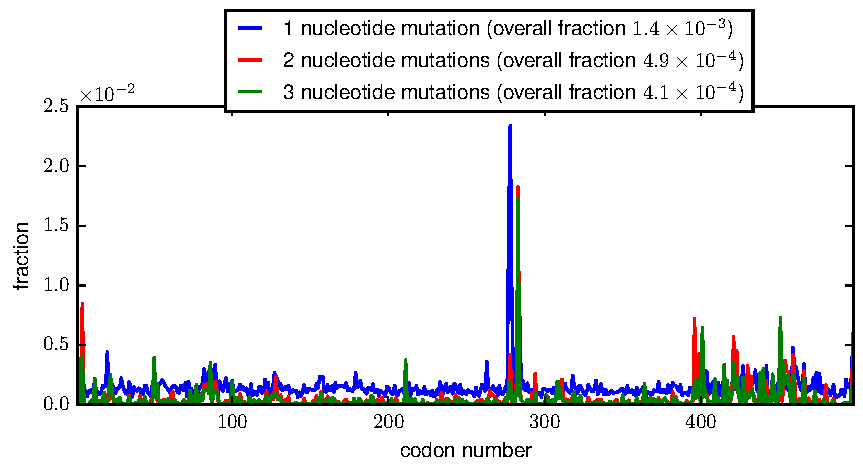
\includegraphics[width=5in]{replicate-1-mutvir_nmutspercodon-dist.pdf}}
\vspace{0.1in}

Fractions calculated using only positions called to the same identity by both paired reads.  Excluded positions for R1 were 1, 2, 3, 4, 5, 6, 7, 8, 9, 10, 11, 12, 13, 14, 15. 
 Excluded positions for R2 were 1, 2, 3, 4, 5, 6, 7, 8, 9, 10, 11, 12, 13, 14, 15. 

\end{document}
